\section{System GSM}
\label{GSM}

Poniższy podrozdział powstał na podstawie źródeł \cite{GSM}, \cite{GSM_tutorialspoint} oraz \cite{GSM_wiki}.\\

System GSM (\textit{ang. \textbf{G}lobal \textbf{S}ystem for \textbf{M}obile Communication}) jest obecnie najpowszechniej stosowanym systemem służącym do komunikacji bezprzewodowej dalekiego zasięgu. Wykorzystywany jest powszechnie do przesyłania głosu oraz serwisów danych. Pomysł na stworzenie sieci umożliwiającej komunikację głosową wyłonił się we wczesnych latach 70. ubiegłego wieku z opracowywanej w siedzibie Bell Laboratories mobilnej sieci radiowej. Jednakże dopiero dwanaście lat później, w 1982 roku powstał oficjalny komitet normalizacyjny nazwany \textit{Groupe Spécial Mobile}, którego zadaniem było utworzenie jednolitego, otwartego standardu dla telefonii komórkowej. 

Pierwotna wersja standardu działała w paśmie 900 MHz (880 - 960 MHz) i umożliwiała jedynie transmisję głosową. Jego kolejna wersja została opublikowana w 1990r. i definiowała ona dodatkowe pasmo 1800 MHz (1710 - 1880 MHz). Ponadto, umożliwiała przesyłanie krótkich wiadomości SMS (\textit{ang. \textbf{S}hort \textbf{M}essage \textbf{S}ystem}), a także faxu czy transmisję danych. Dalsze prace nad systemem wprowadziły do standardu techniki zwiększające przepustowość transmisji (maksymalna prędkość odbioru - 57.6 kb/s, maksymalna prędkość nadawania - 14.5 kb/s) oraz mechanizm przesyłania danych w pakietach GPRS (\textit{ang. \textbf{G}eneral \textbf{P}acket \textbf{R}adio \textbf{S}ervice}) z przepustowością 30 - 80 kb/s). 

Pomimo pojawienia się na świecie nowszych rozwiązań, takich jak sieci UMTS i LTE, ze względu na ogromną popularność, architektura sieci GSM wciąż jest rozwijana. 

System GSM umożliwia skorzystanie z następujących usług:
\begin{itemize}
	\item Połączenia głosowe - Stanowią one sztandarową funkcjonalność sieci GSM. Jej standard definiuje kodek GSM, który służy do zamiany głosu (skonwertowanego przez mikrofon do napięciowego sygnału analogowego) na postać cyfrową, która jest następnie kompresowana stratnie i transmitowana do odbiorcy. Stosowana jest kompresja na podstawie algorytmu LPC (\textit{ang. \textbf{L}inear \textbf{P}redictive \textbf{C}oding}). Po stronie odbiorcy sygnał jest dekodowany, lecz ze względu na stratność LPC, słyszalny jest zniekształcony, nienaturalny głos rozmówcy.
	\item Transmisja danych - Umożliwia dostęp do internetu z urządzenia GSM, a także korzystanie z transmisji strumieniowej.
	\pagebreak
	\item Wiadomości tekstowe i multimedialne - Usługa przesyłania krótkich wiadomości tekstowych, o długości do 160 znaków, pod warunkiem korzystania jedynie z alfabetu łacińskiego. W przypadku stosowania znaków diakrytycznych maksymalny rozmiar wiadomości spada do 70 znaków. Wiadomości multimedialne (inaczej MMS), umożliwiają przesyłanie zdjęć, filmów czy dźwięków. Ich rozmiar maksymalny jest uzależniony od ograniczeń telefonu oraz operatora.
\end{itemize}

Jednym z głównych założeń systemu jest możliwość korzystania z niego przez wielu użytkowników jednocześnie. Aby rozwiązać ten problem, postanowiono zastosować technikę zmiany częstotliwości FDMA (\textit{ang. \textbf{F}requency \textbf{D}ivision \textbf{M}ultiple \textbf{A}ccess}) oraz okien czasowych TDMA (\textit{ang. \textbf{T}ime \textbf{D}ivision \textbf{M}ultiple \textbf{A}ccess}). Oznacza to, że pasmo częstotliwości GSM jest podzielone na wąskie kanały, o szerokości 200 kHz każdy. Czas użytkowania każdego kanału podzielony jest na 8 okien czasowych. Każde urządzenie ma zatem dostęp do sieci dostrajając się do odpowiedniego kanału w czasie trwania przydzielonego okna czasowego. Przedstawiono to na rysunku \ref{fig:image_gsm_frequencies_timeslots}.

\begin{figure}[H]
	\centering
	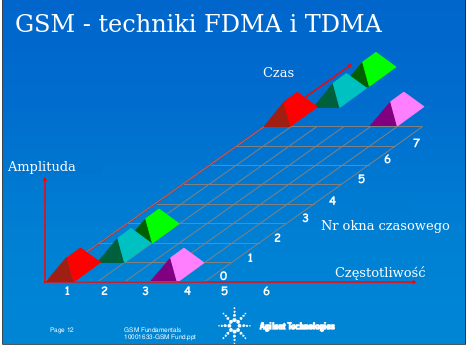
\includegraphics[width=8cm]{img/theory/GSM/gsm_timeslots_frequencies.png}
	\caption{Podział pasma częstotliwości na kanały i okna czasowe. Źródło: \cite{GSM}}
	\label{fig:image_gsm_frequencies_timeslots}
\end{figure}


Architektura sieci GSM powstała w oparciu o komórkowy system radiowy, skąd powszechnie stosowana nazwa - sieć komórkowa. Charakteryzuje się ona tym, że obszar terenu, na którym ma być prowadzona komunikacja radiowa dzieli się na tzw. komórki. Każdej komórce przypisana jest stacja bazowa (\textit{ang. \textbf{B}ase \textbf{T}ranceiver \textbf{S}tation}), która stanowi bramę dostępową do sieci. Urządzenie mobilne GSM, takie jak na przykład telefon, znajdując się na obszarze komórki najczęściej odbiera sygnał z więcej niż jednej stacji bazowej, jednakże zawiera połączenie z tą, której sygnał jest najsilniejszy. W razie spadku mocy sygnału stacji z którą urządzenie jest połączone, możliwa jest dynamiczna zmiana połączenia do innego BTS'a.

\begin{figure}[H]
	\centering
	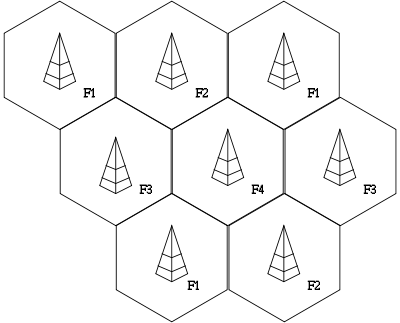
\includegraphics[width=8cm]{img/theory/GSM/cell_structure.png}
	\caption{Podział obszaru na komórki. Źródło: \cite{GSM_wiki}}
	\label{fig:image_gsm_cells}
\end{figure}

Aby móc korzystać z sieci GSM, urządzenia muszą posiadać kartę SIM (\textit{ang. \textbf{S}ubscriber \textbf{I}dentification \textbf{M}odule}). Oprócz przydatnych dla użytkownika wbudowanej pamięci na wiadomości SMS i kontakty, posiada ona unikalny na całym świecie numer identyfikujący użytkownika w sieci. W celu zalogowania się do sieci, urządzenie GSM musi podać ten numer w trakcie nawiązywania połączenia ze stacją bazową. 

Każda stacja bazowa wykorzystuje wiele kanałów GSM. Jednakże, aby nie dopuścić do wzajemnego zakłócania się, stacje bazowe z przylegających do siebie cel wykorzystują inne ich zestawy. Dodatkowo, w stacjach bazowych stosuje się dwa rodzaje anten - dookólne i kierunkowe o pokryciu 120\degree. Anteny dookólne pokrywają caly obszar komórki tym samym zbiorem kanałów, natomiast kierunkowe - dla każdego podobszaru wykorzystują ich inny zestaw. Ze względu na skończoną prędkość sygnału radiowego, istnieje również maksymalny promień pojedynczej komórki. W praktyce wynosi on około 35 km. Poniważ istnieje konieczność umożliwienia prowadzenia komunikacji na tak duży zasięg, standard ten nie należy do najbardziej energooszczędnych. W zależności od klasy urządzenia, minimalna moc nadawajnika może wynosić od 1 do 20 mW, natomiast maksymalna nawet do 8 W. Urządzenia GSM mają możliwość dostosowywania mocy transmisji na podstawie mocy sygnału odebranego od stacji bazowej, w celu ograniczenia wysokiego zużycia energii. 

Biorąc jednak pod uwagę fakt, iż transmisja przebiega w oknach czasowych, moc średnia jest niższa. Każde okno czasowe trwa 577 $\mu s$, a w jego czasie można wysłać jedną z kilku ramek komunikacyjnych. W trakcie każdej z nich można wysłać 148 bitów danych. W przypadku ramki nadawanej w trakcie rozmowy, głos kodowany jest jedynie na 57 bitach. Każde z urządzeń w sieci otrzymuje okno czasowe co 4.615 ms, liczone od początku okna, do rozpoczęcia następnego. Stąd wynika, że w trakcie pojedynczego cyklu nadawania, urządzenie transmituje dane jedynie przez 12.5\% czasu. Dla przykładu, pobór prądu przez moduł GSM zastosowany w pracy, w zależności od odległości do nadajnika, a więc od mocy nadawania, może wówczas wynosić nawet do 1.5 A. Przyjmując napięcie zasilania układu GSM wynoszące 4 V, maksymalna pobierana moc średnia może wynosić:

\begin{gather}
 	P_{\text{śr}} = U \cdot I \cdot \tau \\
 	P_{\text{śr}} = 4 V \cdot 1.5 A \cdot 0.125 = 0.75 W \nonumber 	
 	\label{eq_gsm_power_mean} 
\end{gather}
 gdzie:
 
 $P_{\text{śr}} $ - moc średnia
 
 $U$ - napięcie zasilania układu,
 
 $I$ - nateżęnie prądu w momencie transmisji
 
 $\tau$ - współczynnik wypełnienia impulsu (czas trwania okna czasowego podzielony przez czas pomiędzy oknami czasowymi)
 
Wartość mocy średniej wynosząca 0.75 W odpowiada ciągłemu zużyciu prądu rzędu 187.5 mA przy napięciu zasilania układu rzędu 4 V. 


